\documentclass[a4paper, 12pt]{article}
\usepackage{geometry}
\geometry{a4paper,
total={170mm,257mm},left=2cm,right=2cm,
top=2cm,bottom=2cm}

\usepackage{mathtext}
\usepackage{amsmath}
\usepackage[T2A]{fontenc}
\usepackage[utf8]{inputenc}
\usepackage[english,russian]{babel}
\usepackage{graphicx, float}
\usepackage{tabularx, colortbl}
\usepackage{caption}
\captionsetup{labelsep=period}

\newcommand{\parag}[1]{\paragraph*{#1:}}
\DeclareSymbolFont{T2Aletters}{T2A}{cmr}{m}{it}
\newcounter{Points}
\setcounter{Points}{1}
\newcommand{\point}{\arabic{Points}. \addtocounter{Points}{1}}
\newcolumntype{C}{>{\centering\arraybackslash}X}

\author{Калинин Даниил,\\Мельникова Юлия,\\Б01-108}
\date{\today}
\title{Лабораторная работа 5.1.2. Эффект Комптона}

\begin{document}
\maketitle
\parindent=0cm

\parag {Цель работы}
с помощью сцинтилляционного спектрометра исследуется энергетический спектр $\gamma$-квантов, рассеянных на графите. Определяется энергия рассеянных $\gamma$-квантов в зависимости от угла рассеяния, а также энергия покоя частиц, на которых происходит комптоновское рассеяние.


\parag {В работе используются}
\begin{itemize}
		\item Источник $\gamma$-излучения $^{137}$Cs в свинцовом коллиматоре
		
        \item Фотоэлектронный умножитель на градуированном подвижном кронштейне $\Delta = \pm 1^\circ$ 
		
        \item Компьютер с 10-разрядным АЦП $\Delta = \pm 1$ канал
\end{itemize}

\parag {Экспериментальная установка}~\\
Источником излучения служит $^{137}$Cs, испускающий $\gamma$-лучи с энергией 662 кэВ. Он помещен в толстенный свинцовый контейнер с коллиматором. Сформированный коллиматором узкий пучок $\gamma$-квантов попадает на графитовую мишень 2 (цилиндр диаметром 40 мм и высотой 100 мм.)
	
\begin{figure}[h!]
    \centering
    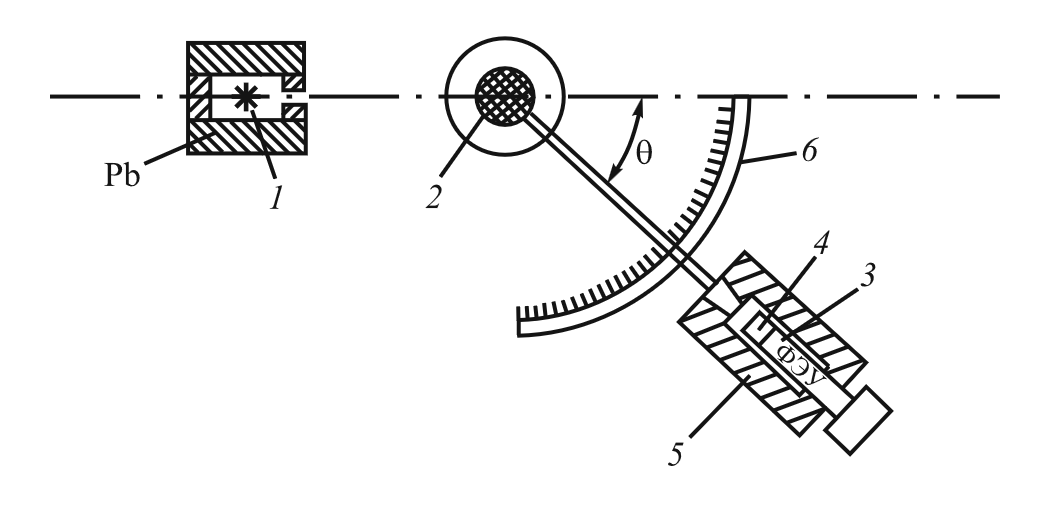
\includegraphics[width=14cm]{ust.png}
    \caption{Экспериментальная установка.}
    \label{fig:ust}
\end{figure}

Кванты, испытавшие комптоновское рассеяние в мишени, регистрируются сцинтилляционным счетчиком. Счетчик состоит из фотоэлектронного умножителя 3 (далее ФЭУ) и сцинтиллятора 4. Сцинтиллятором служит кристалл NaI(Tl) цилиндрической формы диаметром 40 мм и высотой 40 мм, его выходное окно находится в оптическом контакте с фотокатодом ФЭУ. Сигналы, возникающие на ФЭУ, подаются на ЭВМ для амплитудного анализа. Кристалл и ФЭУ расположены в светонепроницаемом блоке, укрепленном на горизонтальной штанге. Штанга вместе с этим блоком может вращаться относительно мишени, угол поворота отсчитывается по лимбу 6.
	
На Рис.~\ref{fig:ust} представлена функциональная блок-схема измерительного комплекса, который состоит из ФЭУ, питаемого от высоковольтного выпрямителя ВСВ, обеспечивающего работу ФЭУ в спектрометрическом режиме, усилителя-анализатора УА, являющегося входным интерфейсом ЭВМ, управляемой с клавиатуры КЛ. В ходе проведения эксперимента информация отражается на экране дисплея Д, окончательные результаты в виде таблиц и графиков могут быть выведены на принтер ПР.

\parag {Экспериментальные данные} ~\\
    \begin{table}[h]
    \centering
        
    \begin{tabular}{|c|c|c|c|}
        \hline
        $\theta$, $^\circ$ & $\sigma_\theta$, $^\circ$ & $N$ & $\sigma_N$ \\ \hline


        0	&	1	&	792	&	10	 \\ \hline
        10	&	1	&	798	&	10	 \\ \hline
        20	&	1	&	687	&	10	 \\ \hline
        30	&	1	&	671	&	20	 \\ \hline
        40	&	1	&	620	&	20	 \\ \hline
        50	&	1	&	555	&	20	 \\ \hline
        60	&	1	&	479	&	20	 \\ \hline
        70	&	1	&	414	&	25	 \\ \hline
        80	&	1	&	361	&	25	 \\ \hline
        90	&	1	&	343	&	25	 \\ \hline
       100	&	1	&	304	&	25	 \\ \hline
       
         
    \end{tabular}

    \label{tab:data}
    \caption{Измеряемые величины и их погрешность.}
    \end{table}

\parag {Ход работы} ~\\
Оценим погрешности величин $1 - \cos \theta$ и $1/N$ по следующим формулам:
\begin{equation*}
    \sigma_{1-\cos \theta} = \sin \theta \cdot \sigma_\theta, \ \sigma_{1/N} = 1/N^2 \cdot \sigma_N.
\end{equation*}
    
Результаты вычислений представлены в Таблице \ref{table:data}:

\begin{table}[H]
    \centering
    \begin{tabular}{|c|c|c|c|}
        \hline
        $1 - \cos \theta$ & $\sigma_{1-\cos \theta}$ & $1/N \cdot 10^3$ & $\sigma_{1/N}$ \\ \hline
        0.000	&	0.000	&	1.263	&	0.040	 \\ \hline
        0.015	&	0.003	&	1.253	&	0.039	 \\ \hline
        0.060	&	0.006	&	1.456	&	0.053	 \\ \hline
        0.134	&	0.009	&	1.490	&	0.056	 \\ \hline
        0.234	&	0.011	&	1.613	&	0.065	 \\ \hline
        0.357	&	0.013	&	1.802	&	0.081	 \\ \hline
        0.500	&	0.015	&	2.088	&	0.109	 \\ \hline
        0.658	&	0.016	&	2.415	&	0.146	 \\ \hline
        0.826	&	0.017	&	2.770	&	0.192	 \\ \hline
        1.000	&	0.017	&	2.915	&	0.212	 \\ \hline
        1.174	&	0.017	&	3.289	&	0.271	 \\ \hline
    \end{tabular}
    \caption{Обработанные данные.}
    \label{table:data}
\end{table}

Изобразим экспериментальные результаты (табл.~\ref{table:data}) в виде графика (рис. \ref{graph:angular}). Согласно теории, экспериментальные точки должны лежать на одной прямой, что, как видно, выполняется с хорошей точностью. Пересечение этой прямой с осью ординат определяет наилучшее значение $N(0)$, а пересечение линии $1 - \cos \theta = 1$ позволяет найти наилучшее значение $N(90)$. 

\begin{figure}[h]
    \centering
    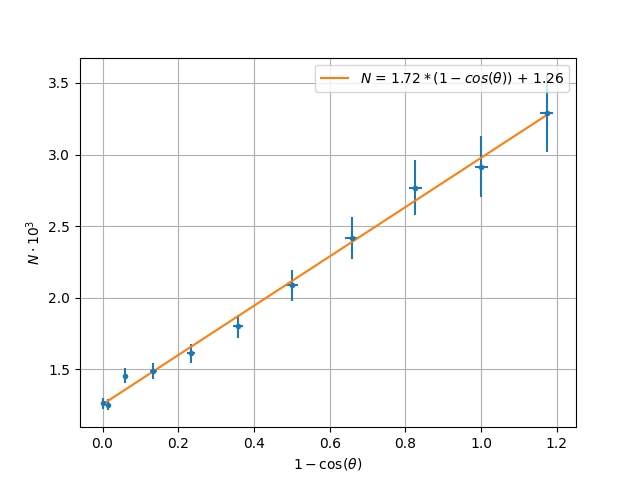
\includegraphics[width=0.8\textwidth]{plot.png}
    \label{graph:angular}
\end{figure}

\parag {Заключение} ~\\
    В лабораторной работе нами была проведена проверка соотношения Комптона. Экспериментально установлено, что $\gamma$-кванты действительно испытывают упругое рассеяние на свободных частицах. 
	
	Обратим наше внимание на то, что с увеличением угла $\theta$ погрешность измерения номера канала $\sigma_N$ увеличивается, что связано со смещением фотопика в сторону сплошного распределения, обязанного комптоновскому рассеянию. При $\theta = 110^\circ$ уже было невозможно увидеть пик полного поглощения.
	
	На основании таблицы \ref{table:data} можно определить энергию покоя частиц, на которых происходит комптоновское рассеивание. Путем несложных преобразований получаем:

	\begin{equation*}
		mc^2 = E(0) \frac{N(90)}{N(0)-N(90)},
	\end{equation*}
	
    где $E(0)$ -- энергия $\gamma$-лучей, испускаемых источником (в нашем случае $^{137}$Cs), то есть 662 кэВ. Имеем:
	\[
	\boxed{mc^2 = 481 \pm 20 \ \text{кэВ}}.
	\]
	Видно, что результат на 6\% меньше 511 кэВ -- энергии покоя электрона. 

\end{document}
